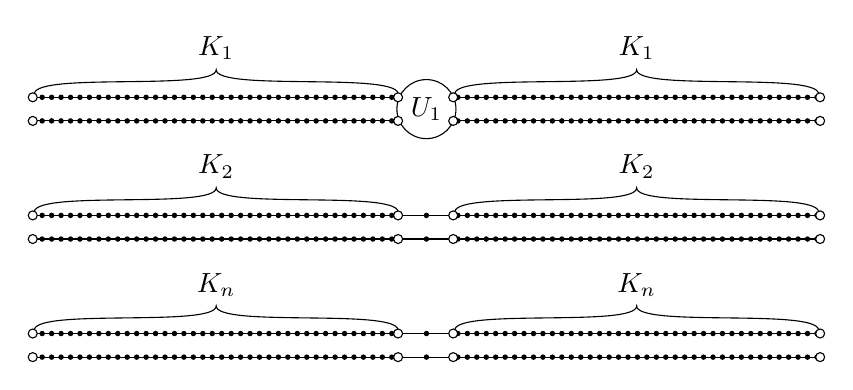
\begin{tikzpicture}[
  unitary/.style={circle,draw=black,fill=white,
    inner sep=0pt,minimum size=7.5mm},
  dots/.style={circle,fill=black,
    inner sep=0pt,minimum size=1.5pt},
  vert/.style={circle,fill=black,
    inner sep=.7pt,minimum size=0pt},
  attach/.style={circle,draw=black,fill=white,inner sep=1.15pt,minimum size=0}]

  \foreach \n /\y in {U_1/3,U_2/1.5,U_n/0}{
    \begin{scope}[yshift = \y cm]
      \foreach \x in {0,.12,...,10} {
        \node at (\x, -.15) [vert] {};
        \node at (\x, .15) [vert] {};
      }
      \draw[fill=white,draw=white] (4.64,-.2) rectangle (5.34,.2);
      \draw (0, -.15) to (10, -.15);
      \draw (0,  .15) to (10,  .15);

    \end{scope}
  }
  
  
      \node at (5,3) [unitary]{$ U_1 $};
      
      \foreach \y in {-.15,.15,1.35,1.65}{
        \node at (5,\y) [vert]{};
      }
  
  \foreach \x in {0,5.34}{
  \foreach \y /\p in {3/1,1.5/2,0/n}{
  \begin{scope}[xshift=\x cm,yshift=\y cm]
    \node (\x\p) at (2.33,.5)[above] {$K_{\p}$};
  
    \draw (0.02,0.2) to[out=80,in=-90,looseness=0.3] (2.33,.5)
                     to[out=-90,in=100,looseness=0.3] (4.64,.2);
  \end{scope}}} 
                  
%  \draw (10.15,2.75) to[out=0,in=-180,looseness=0.3] (10.45,1.25)
%                    to[out=-180,in=0,looseness=0.3] (10.15,-.25);
%  \node at (11.9,1.25)
%      {\begin{tabular}{c}
%          Computational\\ 
%          Qubits\end{tabular}};
%
%
%  \draw (-1,3) to (0, 3) to (0,-2.5) to (-1,-2.5) [dashed];
%  \draw (13.5,3) to (10,3) to (10,-2.5) to (13.5,-2.5) [dashed];
%
%  \node at (5,.9) [dots] {};
%  \node at (5,.75)    [dots] {};
%  \node at (5,.6) [dots] {};
%
%  \draw (10.15,-1.75) to[out=0,in=-180,looseness=1.5] (10.45,-2)
%                    to[out=-180,in=0,looseness=1.5] (10.15,-2.25);
%  \node at (11.9,-2) 
%      {\begin{tabular}{c}
%          Mediator\\ 
%          Qubit\end{tabular}};
          
   \foreach \x in {0, 10, 4.64, 5.34}{
   \foreach \y in {2.85,3.15,1.65,1.35,.15,-.15}{
     \node at (\x, \y) [attach] {};
   }}
\end{tikzpicture}